\documentclass[conference,10pt]{IEEEtran}
\usepackage[T1]{fontenc}
\usepackage{amsmath,amssymb,amsthm,booktabs,array,microtype}
\usepackage[hidelinks]{hyperref}
\usepackage{balance}
\usepackage{placeins}
\newcommand{\DoNotLoadEpstopdf}{}
\usepackage{tikz}
\usetikzlibrary{arrows.meta,positioning}
\newcommand{\G}{\mathsf{G}}\newcommand{\F}{\mathsf{F}}
\newcommand{\CPre}{\operatorname{CPre}}\newcommand{\Pref}{\operatorname{Pref}}
\newcommand{\EPre}{\operatorname{EPre}}\newcommand{\code}[1]{\texttt{#1}}
\newtheorem{theorem}{Theorem}\newtheorem{proposition}[theorem]{Proposition}
\newtheorem{corollary}[theorem]{Corollary}\newtheorem{lemma}{Lemma}
\newcolumntype{L}[1]{>{\raggedright\arraybackslash}p{#1}}
\title{Continuation Preservation in Boolean-Helper Synthesis for Controller Replacement}
\author{\IEEEauthorblockN{Anonymous authors}}
\begin{document}\raggedbottom\maketitle
\begin{abstract}
Controller replacement after an environment-model change must account
for the current state and unfinished obligations. A negative synthesis
result may concern an auxiliary encoding rather than the source contract;
a positive existence result may still yield an unsuitable controller.
We characterize exactly which strict-winning continuations survive a
one-way Boolean-helper encoding, including constraints retained during
translation. If the helper's first change releases input restrictions
before response restrictions, winning requires maintaining the ability
to answer every newly legal input. For one unchanged public Vehicle input,
a whole-region audit of two saved native strict results finds 1,408 source
states that lose strict-winning continuations. Each state is reachable
under some initialized cooperative policy; both initial judgments remain
positive. In a constructed Patrol update, a reusable source controller
coexists with exclusion of its retained entry from the exported encoding.
A complete countercertificate and reduced native query establish this
temporal loss; the full-helper query remains UNKNOWN. A reconstructed Lift example separately
shows why a solved game does not certify a particular extracted graph.
Existing cooperative synthesis after normalization to a total arena supplies
admitted alternatives for the feasible contracts in our fixed rosters. The results clarify the evidence required to retain a contract and admit
a replacement controller.
\end{abstract}
\begin{IEEEkeywords}
self-adaptive systems, reactive synthesis, specification repair,
non-conflicting strategies, controller verification
\end{IEEEkeywords}

\section{Introduction}\label{sec:intro}
A revised map does not erase a robot's pending charging request.
Its current position and request history constrain replacement:
restarting the specification would discard an obligation. Adaptation
must decide whether the requirements still admit a continuation and
which controller can be installed from that context~\cite{specrepair,degradation,dupdate}.

A tool translates the contract, solves the encoded game and extracts a
controller (Fig.~\ref{fig:evidence-overview}). Two decisions follow.
First, if the encoding preserves source continuations at the retained
entry, a correct strict solver's negative result there rules them out.
Second, installation requires auditing the returned graph at that source
state and selected private root; an existence result alone does not
certify it.

\begin{figure*}[t]
\centering
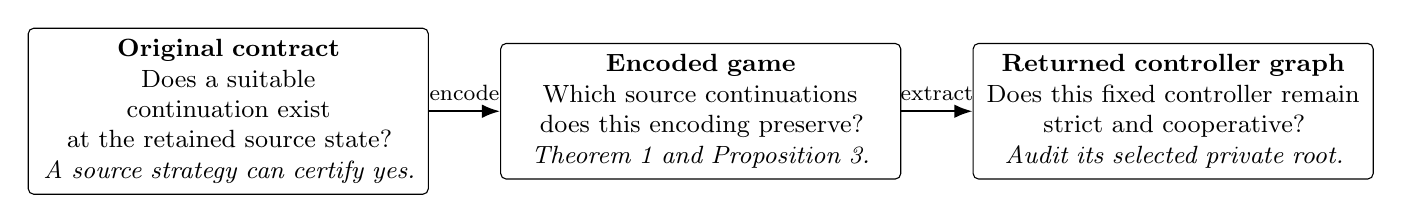
\begin{tikzpicture}[>=Latex,every node/.style={font=\small,align=center},
box/.style={draw,rounded corners=2pt,text width=4.8cm,minimum height=1.7cm,inner sep=4pt}]
\node[box] (source) at (0,0) {\textbf{Original contract}\\Does a suitable continuation exist\\at the retained source state?\\\emph{A source strategy can certify yes.}};
\node[box] (game) at (6.0,0) {\textbf{Encoded game}\\Which source continuations\\does this encoding preserve?\\\emph{Theorem 1 and Proposition 3.}};
\node[box] (graph) at (12.0,0) {\textbf{Returned controller graph}\\Does this fixed controller remain\\strict and cooperative?\\\emph{Audit its selected private root.}};
\draw[->,thick](source.east)--node[above,font=\footnotesize]{encode}(game.west);
\draw[->,thick](game.east)--node[above,font=\footnotesize]{extract}(graph.west);
\end{tikzpicture}
\caption{Evidence needed for a state-preserving replacement. An encoded
strict refusal transfers to the original contract only with preservation
at the same entry. A failed returned graph excludes that graph; it does
not exclude every source strategy. Source state and logical obligations
are retained, while each candidate binds its own private root.}
\label{fig:evidence-overview}
\end{figure*}


We study a one-way Boolean-helper encoding that releases environmental
safety before system safety on its first change. Newly legal inputs can
require incompatible responses. Preservation requires answering them
throughout a winning continuation, beyond a one-step check at the entry.

Our exact characterization (Theorem~\ref{hpb:exact}) extends to retained
translation constraints (Proposition~\ref{hpb:retained}) and gives a
necessary-and-sufficient condition for preserving the entire original
strict-winning region. The complete first-flip correction already
exists~\cite{spectrarelease2024}; our contribution characterizes the
other encodings.

Vehicle exposes initialization's blind spot: two completed native strict
queries preserve both initial judgments but lose source continuations.
This public input is outcome-selected; initialized cooperative
reachability is existential per target. Patrol exposes the local check's
blind spot: a reusable source controller coexists with temporal encoding
loss. A countercertificate and reduced native query establish it; the
full-helper query remains UNKNOWN. Lift addresses installation: a solved
game yields an unsuitable fixed graph. Its selection intervention is a
diagnosis, not a general repair.

Existing normalized synthesis supplies admitted alternatives in the fixed
rosters; Patrol has an audited reusable controller. Certified source
continuations can thus justify retaining requirements despite encoding
or output failure, without establishing deployment frequency or superiority.

We define replacement, prove preservation, diagnose both boundaries, and
report admission and comparisons in Sections~\ref{sec:running-example}--\ref{sec:replication}.
The public artifact groups the paper, claim evidence, tool sources and
scoped replay instructions by purpose~\cite{artifactrepository}.

\section{The Replacement Decision and Its Semantics}\label{sec:running-example}
The update boundary retains the full source state $r$, including logical
history monitors for unfinished obligations. The \emph{original contract}
is the candidate after the proposed environment change or repair, before
adding synthesis auxiliaries. A replacement graph may select a new private
root; it must match $r$ rather than restart the original initializer.
Checking assumes a valid holding state until installation. A changing
physical state instead needs a verified update bridge or revalidation.

\paragraph{Source continuations}
Its finite, fully observed Mealy game $M$ has nonempty typed input and
response carriers $E,Y$, with states $D=E\times Y$. A round starts at
$s=(e,y)$: ENV supplies the next input $e'$, SYS observes it and chooses
$y'$, and the next state is $s'=(e',y')$. Environmental safety is
$\rho_e(s,e')$, independent of the next response; system safety
$\rho_s(s,e',y')$ includes every system constraint and logical-monitor
update. Neither relation need be total. Initial predicates are
$\theta_e(e)$ and $\theta_s(e,y)$; invalid type encodings are outside $D$.

Safety specifies allowed steps. A justice condition must hold
infinitely often; the ENV and SYS lists define generalized B\"uchi
objectives $A$ and $G$. Under \emph{strict} semantics~\cite{gr1,kind},
SYS must satisfy safety while the ENV safety prefix, including the
current edge, holds, and must satisfy $A\Rightarrow G$ on infinite
safety-compliant plays. An ENV safety violation releases the safety
duty on that edge and thereafter. Unfairness cannot excuse an earlier
required safety violation. Strategies retain private memory and give
typed responses even to illegal inputs.

An original-legal prefix follows the declared entry and original safety
relations. A fixed strategy is \emph{legal-prefix cooperative} if every
such prefix admits an infinite environment-safe continuation satisfying
all ENV justices, with that same strategy and reached memory~\cite{cooperative,friendly}.
For a strict strategy, this continuation also satisfies SYS justice.
Thus a legal next input is necessary but insufficient: a controller
may leave inputs available while preventing a required event forever.

Kind's Definition~3~\cite{kind} includes illegal strategy-consistent
histories; our positive certificates establish legal-prefix cooperation.
Neither resets reached memory. A failure on a legal prefix also refutes
the stronger property for that output, but does not exclude every strategy.

Let $W$ contain source states admitting some strict-winning continuation,
and $K$ those admitting some strict, legal-prefix cooperative continuation. These regions quantify over
strategies and their memory. More generally, $\operatorname{Win}_{\rm str}(N)$
denotes states with a strategy satisfying the strict duties of game $N$
against every environment strategy. The regions include unreachable typed states and
are independent of initialization; $W$ may include environmental dead
ends through strict vacuity. An active continuation has already met ENV
initialization, prior safety, and required SYS duties.

\paragraph{What each result licenses}
An entry is \emph{preserved for strict winning} when original winning at
$r$ implies winning at its corresponding encoded state. With a correct
strict solver, this implication permits a negative encoded result to
exclude $r\in W$. Without it, an encoded refusal leaves source feasibility
unresolved. A cooperative-core result needs its own sound correspondence;
it cannot automatically be read as a strict-game result.

A returned graph fixes private memory $q$ as well as source state $s$.
Its admission check binds a particular $(r,q)$ and verifies every
original-legal branch, safety, liveness and cooperation. A passing graph
is a constructive feasibility certificate and may be installed under the
holding assumption. A failing graph excludes that candidate, not all
source strategies. Section~\ref{sec:replication} gives the complete checks.


\section{Exact Continuation Preservation}\label{sec:formal}
We now characterize the encoding's strict-winning region. The fresh
Boolean input $b$ is observed before SYS responds, starts false, and can
change to true only once. The added assumption $\G\F\neg b$ makes an
infinite play after the change unfair, but does not excuse an earlier
strict-safety violation. We distinguish a response possible now ($C$) from maintaining
that condition while winning ($W_C$), then treat retained constraints.

\begin{samepage}
\paragraph{The literal reduction}
Kind prints each safety assumption as
$\rho_n^e\lor\operatorname{next}(\mathit{envHelp})$ and each safety
guarantee as $\rho_n^s\lor\mathit{envHelp}$~\cite[Sec.~4.1]{kind}.
Writing $b=\mathit{envHelp}$, conjoining the complete clauses and
including helper persistence gives
\begin{align}
 \theta_e^R &= \theta_e\land\neg b,
 &\theta_s^R &= \theta_s, \nonumber\\
 \rho_e^R &= (\rho_e\lor b')\land(\neg b\lor b'),
 &\rho_s^R &= \rho_s\lor b, \label{hpb:literal}\\
 A^R &= A\land\mathbf{G}\mathbf{F}\neg b,
 &G^R &= G. \nonumber
\end{align}
\end{samepage}
Write $W_R(s,b)$ for the transformed strict-winning predicate.
The \emph{complete-relation hypothesis} means that the guards apply to
the entire safety relations, including every logical auxiliary constraint.
It must be checked for a syntactic route after all translations.

With $b=b'=0$, both original safety relations apply; with $b=b'=1$,
both are released. A helper-false non-flip input violates transformed
ENV safety exactly when it violates original ENV safety.
The mismatch occurs on the first flip, $b=0,b'=1$:
any typed $e'$ is allowed, including one disallowed by $\rho_e$,
while $\rho_s$ still applies. Define
\begin{equation}
 C(s)\ \equiv\ \forall e'\in E\ \exists y'\in Y:
                    \rho_s(s,e',y').
 \label{hpb:C}
\end{equation}
There is no environmental-safety antecedent in $C$. This is a local
response test; $W_C$ requires a source strategy that maintains $C$ while
satisfying the original strict duties.
Let $M_C$ have the original environmental relations and justice
objectives, but system safety
\begin{equation}
 \rho_s^C(s,e',y')\ \equiv\
 C(s)\land\rho_s(s,e',y')\land C(s').
 \label{hpb:C-invariant}
\end{equation}
With $\operatorname{Win}_{\mathrm{str}}$ denoting the strict-winning
region of its argument game, define
$W_C=C\cap\operatorname{Win}_{\mathrm{str}}(M_C)$ independently
of initialization. The outer intersection excludes outside-$C$
states winning vacuously at environmental dead ends.

\paragraph{Why a response now is not enough}
The patrol update of Section~\ref{sec:patrol} changes only ENV, so the
immediate response condition $C$ is unchanged and holds at the pending
entry. The new environment can nevertheless force a later charging
state outside $C$, even though a strict cooperative source controller
still exists. Surviving the conversion therefore requires a strategy
that maintains $C$ through future legal steps.


\begin{samepage}
\begin{theorem}[Exact strict-winning continuation region]
\label{hpb:exact}
Under the stated Mealy, strict, and complete-relation hypotheses,
the reduction~\eqref{hpb:literal} has, for every $s\in D$,
\begin{equation}
 W_R(s,0)=W_C(s),\qquad W_R(s,1)=\mathit{true},
 \label{hpb:exact-equation}
\end{equation}
identifying a region with its characteristic predicate.
\end{theorem}
\end{samepage}

\begin{proof}
At $b=1$, legal edges retain the helper, system safety is released,
and every infinite legal play violates $\G\F\neg b$; hence all states win.

For necessity, a winning strategy at $(s,0)$ must answer every legal
first flip $(e',1)$ with a $\rho_s$-safe response, so $s\in C$.
Restrict it to original-legal histories with $b=0$: these have exactly
the original obligations. After each such finite prefix its residual
strategy still wins, because required safety holds and B\"uchi conditions
are prefix-independent. Repeating the first-flip argument gives $C$ at
every reached successor. The restricted strategy therefore wins $M_C$,
so $W_R(\cdot,0)\subseteq W_C$.

Conversely, start from $s\in W_C$ and follow a winning $M_C$ strategy
while $b=0$ and inputs are original-legal. It maintains $C$, which
supplies a safe response to any first flip. The successor has $b=1$
and is winning by the first paragraph. Without a flip, original safety
and liveness coincide; transformed-illegal inputs release strict duties.
Thus $W_C\subseteq W_R(\cdot,0)$.
\end{proof}

\begin{corollary}[Full-region preservation]
\label{hpb:full-preservation}
The literal reduction preserves the entire original strict-winning
region at $b=0$ if and only if $W\subseteq C$.
\end{corollary}
\begin{proof}
$W_C\subseteq W\cap C$ and Theorem~\ref{hpb:exact} give necessity.
If $W\subseteq C$, every original-legal prefix of an original winning
strategy has a winning residual strategy. Every reached state therefore
belongs to $W\subseteq C$, so that strategy satisfies
\eqref{hpb:C-invariant} and wins $M_C$. Hence $W\subseteq W_C$, proving
sufficiency with the reverse inclusion.
\end{proof}

The exact loss $W\setminus W_C$ can exceed $W\setminus C$:
a response possible now may force a later state outside $C$.
The patrol update demonstrates this propagated loss at a reached
entry with a genuinely pending request (Section~\ref{sec:patrol}).

\paragraph{Preservation from the original initializer}
For initialization of $M$ with a continuation region $T$, write
\begin{equation}
 I_M(T)\ \equiv\ \forall e\in E:\theta_e(e)\Rightarrow
 \exists y\in Y:\theta_s(e,y)\land T(e,y).
 \label{hpb:initial}
\end{equation}
Original and transformed initial realizability are $I_M(W)$ and
$I_M(W_C)$, respectively, by Theorem~\ref{hpb:exact} and initial $b=0$.
Since $W_C\subseteq W$, original unrealizability is preserved.
Full-region preservation suffices but is unnecessary for initial
preservation, as the initialized/reached-state contrast in Supplement~E
demonstrates.

\paragraph{When syntactic constraints remain}
Retained constraints add three questions: where can SYS remain safe
after the flip, which states allow safe entry there, and where can a
source winning strategy maintain that entry condition?

Let $E_{ij}(s,e')$, $S_{ij}(s,e',y')$ be the safety relations for helper
transition $i\to j$. Retain all typed variables and logical monitors;
the next helper is observed before the response. Assume
$E_{00}=\rho_e$, $S_{00}=\rho_s$, $E_{10}=\mathit{false}$, and no
next-response dependencies in $E_{ij}$. For generalized B\"uchi objectives
$A',G'$, the transformed objectives are $A'\land\G\F\neg b$ and $G'$ globally, where the corresponding
state predicates of $A',G'$ agree with those of $A,G$ at $b=0$;
they may be arbitrary at $b=1$.
For $Z\subseteq D$, $\CPre_{11}(Z)$ contains the states where every
typed input satisfying $E_{11}$ admits a typed $S_{11}$-safe response
into $Z$; states with no legal input qualify vacuously. Define
\[
\begin{aligned}
U&=\nu Z.\,\CPre_{11}(Z),\\
F&=\{s\mid\forall e'\in E:E_{01}(s,e')\Rightarrow{}\\
 &\qquad\exists y'\in Y:S_{01}(s,e',y')\land(e',y')\in U\}.
\end{aligned}
\]
Let $M_F$ replace system safety by $F(s)\land\rho_s(s,e',y')\land F(s')$,
retaining original environmental relations and justices, and define
$W_F=F\cap\operatorname{Win}_{\mathrm{str}}(M_F)$.
Thus $U$ requires continued safety after a flip, and $F$ requires safe entry.
\begin{proposition}[Preservation with retained constraints]\label{hpb:retained}
Under these hypotheses,
the strict regions are $W_R(\cdot,1)=U$ and $W_R(\cdot,0)=W_F$.
Full preservation holds exactly when $W\subseteq F$; unchanged original
initialization with $b=0$ gives $I_M(W_F)$.
\end{proposition}

\begin{proof}
At $b=1$, persistence keeps the helper true, so the added assumption
fails and only strict safety remains. The fixed point $U$ supplies safe
responses back into $U$; conversely, states with safety-winning residual
strategies form a post-fixed point of $\CPre_{11}$. Thus $W_R(\cdot,1)=U$.

From a winning helper-false state, each legal flip must enter $U$ safely.
The same holds after every original-legal non-flip prefix, so all reached
states satisfy $F$. Restriction to those histories wins $M_F$.
Conversely, from $s\in W_F$, a winning $M_F$ strategy maintains $F$ until a flip, then
enters $U$ and switches to a uniform safety-winning strategy, available
in this finite, fully observed game. Without a flip, original duties
hold; afterwards safety holds and the added assumption fails. Illegal
inputs release strict duties. This proves $W_R(\cdot,0)=W_F$.

Finally, $W_F\subseteq W\cap F$ gives necessity for preservation.
If $W\subseteq F$, every residual state of an original winning strategy
lies in $W$, hence in $F$; that strategy wins $M_F$, proving sufficiency.
The unchanged initializer gives $I_M(W_F)$.
\end{proof}

Uniformity follows from $U=\CPre_{11}(U)$: for each $s\in U$ and
each $E_{11}$-legal input $e'$, fix one safe response into $U$, giving
a common memoryless selector.

Safe entry matters even when a flip response exists. With one input value,
Boolean response $y$, true initial and justice predicates,
$\rho_e=\mathit{true}$ and $\rho_s=y'$, we have $W=C=D$.
Keep $E_{01}=E_{11}=\mathit{true}$ and $S_{01}=y'$, but let
$S_{11}=\neg y\land\neg y'$. Then $U=\{y=0\}$ is proper:
every flip forces $y'=1$ outside $U$, so $F=W_F=\varnothing$.
By contrast, complete literal relations give $U=D,F=C$; the complete
correction below gives $U=F=D$. Supplement~L.1 retains the full example.
The Patrol study below applies this general criterion to actual retained
constraints. Additional public-input checks and the full scope of each
conversion are in Supplement~D. Conditions using $W$ do not provide a
low-cost runtime precheck.

\paragraph{The existing first-transition correction}
A released semantic-reduction class ORs $b$ and $\neg b\land b'$
into SYS safety when ENV safety is not universally true~\cite{spectrarelease2024};
otherwise it skips reduction. This is an existing implementation class,
not an established frontend option or default. Our $R^+$ formalizes this existing rule on complete relations,
replacing only system safety by
\begin{equation}
 \rho_s^{R^+}=\rho_s\lor b\lor b'.
 \label{hpb:corrected}
\end{equation}
For complete relations under the same hypotheses, the first flip and
later helper-true edges release SYS safety: $S_{01}=S_{11}=\mathit{true}$.
Proposition~\ref{hpb:retained} gives $U=F=D$, hence $W_F=W$ and
$W_{R^+}(s,0)=W(s)$. Unchanged initializers with initial $b=0$ preserve
initial realizability. Supplement~L.6, Proposition~L.4 gives the
restriction-and-extension proof.
This special case does not characterize loss under retained syntactic constraints.
\paragraph{Why the exact encoding matters}
Guard has Boolean input $x$, response $y$, true initial and justice
predicates, and $\rho_e=\rho_s=x'$. A constant response is strict-winning;
ENV can choose $x'=1$ forever after any strategy-consistent history,
also satisfying Kind's all-history Definition~3. Yet $C=\varnothing$:
the first-flip input $(x',b')=(0,1)$ is legal and has no safe response.
Thus the complete printed Section~4.1 relations reject this contract.
They differ from the construction in Kind's strict-realizability proof:
Appendix~A instead writes $\rho_e\lor b$, while the separate semantic
implementation uses the preserving correction above~\cite[Theorem~1,
Appendix~A]{kind}. This is a discrepancy among constructions, not a
counterexample to the corrected expression or the separate
well-separation theorem.

The selected released syntactic/JTLV route also reports raw-core
unrealizability on Guard before extraction. Its saved relations independently
show $(0,1)$ legal and $x'\lor b$ false for both responses at every
helper-false initial state~\cite{newartifact}. That certifies strict loss
without treating the raw cooperative-core verdict as a strict result
or claiming a frontend-default execution.

\section{Diagnosing Continuation Loss}\label{sec:evaluation}
Vehicle shows a direct first-flip obstruction with completed native
queries; Patrol shows loss propagated back to an entry that passes the
immediate check. A \emph{route} is a specific translation, solver and
extraction chain. Table~\ref{tab:route-evidence} binds each claim to that
chain, distinguishing saved relation certificates from executed queries.

\begin{table*}[t]
\centering\small
\caption{Binding the principal claims to their source, encoding and query.
``Native'' names an executed tool query, not a frontend observation.
The selected release is Spectra~\cite{spectra} \code{1.0.0.202402072123}/JTLV.
Bindings: Supplements~B, E, U, V and X.}
\label{tab:route-evidence}
\begin{tabular}{@{}L{20mm}L{52mm}L{43mm}L{49mm}@{}}\toprule
Instance & Source and encoded relations & Calculation or producer & Supported conclusion and limit\\\midrule
Vehicle188 & Unchanged public source; full exported syntactic-helper relations match
the complete literal encoding~\eqref{hpb:literal}. &
Two completed full \code{GR1Game} strict queries; independent whole-region evaluation of their saved winning BDDs. &
1,408 of 8,064 source strict/cooperative states lost; both initial judgments true. Cooperation and pointwise initialized reachability use source proofs.\\[3pt]
Patrol new & Unchanged public source; syntactic helper. $E_{00}=\rho_e$,
$S_{00}=S_{01}=\rho_s$; $E_{01}=E_{11}=\top$; $S_{11}$ retains AUX updates. &
Full relation checks; complete countercertificate; explicit and native reduced-game queries. &
Certified $r\in W\setminus W_F$ with $U=D,F=C$. Direct full-helper native queries remain UNKNOWN.\\[3pt]
Lift T & Reconstructed published listing; selected syntactic helper. Original predicates
match the helper-false view; no source clause is repaired. &
Raw \code{GR1SeparatedGame} core; generic finite-memory extraction (named in Supplement~W.2). One solve, two final selections. &
One strict-only graph, one strict cooperative graph. This tests the selected generic extractor, not a historical or default frontend.\\\bottomrule
\end{tabular}
\par\smallskip\raggedright\footnotesize
The headless route applies the syntactic reduction before default
translation and BDD construction, followed by the strict query or the raw,
unnormalized cooperative core with generic extraction. Supplements~Y.1
and W.2 give the implementation chain. Typed-domain BDD comparisons bind
the listed Vehicle/Patrol branches and Lift's helper-false view, including
initializers and ordered justices. The chain is statically mapped to public
Kind; defaults use ordinary GR(1). GUI execution, historical C-driver identity
and a frontend option for the separate semantic correction remain unestablished.
\end{table*}

\subsection{Vehicle: a public reached-state loss with positive initialization}
\label{sec:vehicle}
Unchanged public Vehicle188 supplies a separate, outcome-selected witness.
It lies outside the fixed cohorts in Section~\ref{sec:replication}.
Let $o_i,p_i,g_i$ be lane-$i$ obstacle, pedestrian and green-light
Booleans, $x$ a crosswalk Boolean, $\ell\in\{1,2,3\}$ the lane and
$v\in\{0,\ldots,10\}$ the speed. The source has true initial predicates.
Three relevant source safety clauses are
\[
\begin{aligned}
\mathrm{ENV}:\quad &o_2\Rightarrow(\neg o'_1\lor\neg o'_3),\\
\mathrm{SYS}:\quad &(\ell=2\land o_2\land o'_1)\Rightarrow\ell'=3,\\
& (\ell=2\land o_2\land o'_3)\Rightarrow\ell'=1.
\end{aligned}
\]
These are selected clauses, not the complete safety relations. At
$s=(o,p,g,x;\ell,v)=(010,000,111,0;2,0)$, the original input rule
excludes simultaneous next obstacles in both outer lanes. On the first
helper flip, the typed input $(o',p',g',x')=(101,000,111,0)$ becomes
legal while both response clauses remain active: they require
$\ell'=3$ and $\ell'=1$. No choice of next speed can resolve that conflict.
The current stopped state is allowed: the positive-speed duty's antecedent
includes $\neg o_2$, which is false at $s$.

The two completed full native strict queries in
Table~\ref{tab:route-evidence} confirm $s\in W$ and $(s,0)\notin W_R$,
while both actual initializer judgments are true~\cite{vehicleartifact}.
They use unchanged initializers and no extra transition restriction.
Thus positive initialization can coexist with loss at a reached state.
The strict queries do not compute cooperative strategies or reachability;
those claims use separate source proofs.

\paragraph{The complete continuation region}
A preregistered audit~\cite{vehiclewholeartifact} evaluates all 33,792 typed source states in the
saved native winning BDDs. Two independent saved-BDD evaluators agree:
$|W|=8,064$, the helper-false winning slice contains 6,656 source states,
and exactly 1,408 source winners are lost, with no gains.
\emph{Cooperation from every winning state.}
The other ENV safety clauses are $o_1\Rightarrow\neg o'_2$ and
$o_3\Rightarrow\neg o'_2$; all ENV justices are
$g_i\land\neg p_i\land\neg o_i$. Thus
$e_*=(o,p,g,x)=(000,000,111,0)$ is always legal and can repeat fairly,
independently of SYS. From any legal prefix of any strict-winning policy,
continuing that same policy on $e_*^\omega$ gives a compatible fair
continuation. Hence every such policy is cooperative and $W=K$.

\emph{A safe predecessor for every target.}
For each $s\in W$, fix $p_s=(e_*;\ell(s),1)$. The remaining SYS
safety clauses require current speed zero for a red light or pedestrian
in the occupied lane, positive speed in a free occupied lane, and speed
below five at a crosswalk. They also force lane changes from current
obstacles and forbid direct jumps between lanes 1 and 3. At $p_s$,
the stop, crosswalk and obstacle guards are false; speed 1 meets the
active free-lane duty, and retaining the lane avoids both forbidden
jumps. Next speed has only its type bound. The three ENV safety
antecedents are also false. Thus $p_s\to s$ is safe for every typed target.
The audit separately verifies $p_s\in W$ and its initializer, checking
$\theta_e(p_s)\land\theta_s(p_s)\land W(p_s)\land
\rho_e(p_s,e(s))\land\rho_s(p_s,e(s),y(s))$ for all 8,064 targets.

\emph{An initialized policy for each target.}
All 1,024 initial ENV assignments have a winning SYS response.
Choose $p_s$ at initial input $e_*$; on next input $e(s)$, take the safe
edge and win from $s$, otherwise follow a winning policy from $p_s$.
For other initial inputs, use winning responses and their winning tails.
Every branch wins, so the policy is strict and, by the preceding argument,
cooperative. Its legal play $p_s,s$ reaches $s$ at time~1. The policy may
depend on $s$; neither forced reachability nor one policy visiting all
targets follows. Supplement~X supplies full source checks.

A correct helper controller stays winning along legal executions of its
unchanged game. The
replacement question concerns a retained state not already guaranteed
to lie in the changed candidate's winning region, even when the synthesis
route is unchanged. Vehicle proves source-policy reachability, not a
model-change execution or a frequency estimate.

\subsection{Patrol: strict-winning continuation lost from a pending entry}
\label{sec:patrol}\label{sec:preservation-evidence}
\begin{figure*}[t]
\centering
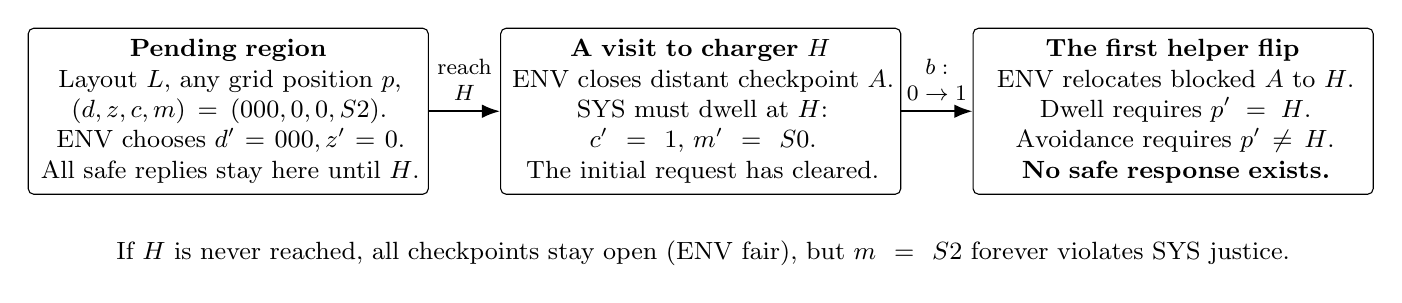
\begin{tikzpicture}[>=Latex,every node/.style={font=\small,align=center},
box/.style={draw,rounded corners=2pt,text width=4.8cm,minimum height=2.05cm,inner sep=4pt}]
\node[box] (pending) at (0,0) {\textbf{Pending region}\\Layout $L$, any grid position $p$,\\$(d,z,c,m)=(000,0,0,S2)$.\\ENV chooses $d'=000,z'=0$.\\All safe replies stay here until $H$.};
\node[box] (exit) at (6,0) {\textbf{A visit to charger $H$}\\ENV closes distant checkpoint $A$.\\SYS must dwell at $H$:\\$c'=1$, $m'=S0$.\\The initial request has cleared.};
\node[box] (flip) at (12,0) {\textbf{The first helper flip}\\ENV relocates blocked $A$ to $H$.\\Dwell requires $p'=H$.\\Avoidance requires $p'\ne H$.\\\textbf{No safe response exists.}};
\draw[->,thick] (pending.east)--node[above,font=\footnotesize]{reach\\$H$}(exit.west);
\draw[->,thick] (exit.east)--node[above,font=\footnotesize]{$b:$\\$0\to1$}(flip.west);
\node[align=center,text width=16.8cm] at (6,-1.8)
{If $H$ is never reached, all checkpoints stay open (ENV fair), but $m=S2$ forever violates SYS justice.};
\end{tikzpicture}
\caption{Countercertificate for the new Patrol encoding: avoid $H$
forever and violate SYS justice, or reach $H$ and face the impossible flip after the initial
request clears. The flip relocation is source-illegal. The published new
source is unchanged; the old restriction, layout and reusable policy
are constructed. Evidence bindings: Table~\ref{tab:route-evidence}.}
\label{fig:patrol-motivation}
\end{figure*}

Patrolling (Kind corpus~277~\cite{kindartifact}) requires a robot on a
$5\times5$ grid to revisit three fixed checkpoints and the origin,
reach charger $(4,0)$ on low power, and dwell for four states. Closure
flags cannot change within one cell; movement avoids blocked checkpoints.
The source requires infinitely many visits to each checkpoint and the
origin, and infinitely many states with $\mathit{request}=S0$.
The three ENV justices require each checkpoint to reopen infinitely
often. The logical request monitor, retained at the update, is $S2$
while the charging request is pending. At the retained entry with helper
false, the complete literal old/new games give win/loss. For the selected
syntactic exports, this comparison is loss/loss with the original old
spelling and win/loss with the equivalent-old-spelling control. The initial
request clears before the obstruction: the loss concerns full strict
continuation. Supplement~S gives all source clauses
and monitor transitions.

The constructed old model fixes layout $L=(A,B,C)=((0,4),(2,4),(4,4))$
and permanent checkpoint availability. Removing these additions yields
the published new source; coordinate persistence retains the reached
layout. SYS requirements, types and monitor equations are identical.
Write $p,d,z,c,m$ for position, blocked flags, charged flag, counter and
logical monitor, and $q$ for private phase. An old BOOT step stays at the
origin and changes $(m,q)=(S0,-1)$ to $(S2,0)$, reaching the source state
\[
 r=(L,p,d,z,c,m)=(L,(0,0),000,0,0,S2).
\]
The controller has private phase $q=0$. The update retains both $r$ and
$q$ without reinitialization.

\paragraph{Source updates}
ENV preserves checkpoint coordinates, freezes a blocked flag within
$\|p-t_i\|_\infty\le1$, and requires $c=3\Rightarrow z'$.
SYS moves at most one cardinal step, avoids each currently blocked
checkpoint's next position, and stays at $H=(4,0)$ while $c<3$.
Its counter update is $c'=\min(3,c+1)$ at current $p=H$, and zero
otherwise. The complete request-monitor update is
\[
 m'=\begin{cases}
 S2,&m=S0,\ \neg z,\ c<3,\ p\ne H,\\
 S1,&m=S2,\ c=3,\\
 S0,&m=S2,\ c<3,\ p=H,\\
 m,&\text{otherwise}.
 \end{cases}
\]
Here $c\in\{0,1,2,3\}$ and every right-hand variable is current.
The absorbing $S1$ remains in the typed arena. A policy reaching $H$
with $(c,m)=(0,S2)$ clears the request on the next dwell, giving
$(c',m')=(1,S0)$ before $c$ reaches three.

\paragraph{A source continuation}
Let $O=(0,0)$, $H=(4,0)$ and standoffs
$s_A=(0,2),s_B=(2,2),s_C=(4,2)$. A handwritten policy expands
\[
\begin{aligned}
O&\to s_A\to A\to s_A\to s_B\to B\to s_B\\
 &\to s_C\to C\to s_C\to s_A\to O\to H\to s_C\to s_A
\end{aligned}
\]
into cardinal unit steps, then resumes the approach to $A$.
On each legal input it holds position and phase if $p=H,c<3$, or
if at a standoff before approaching checkpoint $i$ and $d_i'=1$;
otherwise it advances one step and its private phase. Source counter and
monitor updates apply even during a hold. Reopening fairness ends each
wait; entering the one-cell neighborhood freezes an open flag through
the visit and retreat. This policy was designed after diagnosis as a
controlled reuse witness.

Complete checks establish $r\in K_{\rm old}\cap K_{\rm new}$: the old
initialized closure has two roots, 140 nodes and 277 edges; the new
closure from $r$ with private phase $q=0$ has 849 nodes and 12,240 edges. The old closure stays
in $C$. The new one has 62 nodes outside $C$ but remains legal-prefix
cooperative: relocating flip inputs are source-illegal. Its all-history
Definition~3 status is not established or needed for strict loss. Supplement~S retains the
complete graphs and all source, monitor, memory and justice checks.

\paragraph{A local pass, but an exact continuation loss}
Let $N(s)$ count movement/dwell-permitted next robot cells, and $k(s)$
count currently blocked checkpoints. Neither these constraints nor the
unique AUX updates depend on next charged/blocked flags. The complete
literal flip condition is
\[
 C(s)\quad\Longleftrightarrow\quad N(s)>k(s).
\]
A flip can choose arbitrary typed next checkpoint coordinates, so $k$
blocked checkpoints can cover all $N$ cells exactly when $N\le k$;
counter and monitor updates are unique. The old graph stays in $C$,
proving $r\in W_C^{\rm old}$ for the complete literal relations.
The actual old-source export has a different helper-false ENV relation,
as detailed below. SYS safety is unchanged, so $C(r)$ is true under both
models. Nevertheless, $r\notin W_C^{\rm new}$.

A 26-node countercertificate covers \emph{every safe response},
independently of that policy or private memory. Its 25 nonexit rows are
exactly the states with layout $L$, any grid position $p$, and
$(d,z,c,m)=(000,0,0,S2)$. Away from $H$, ENV keeps the flags open and
power low. Every safe reply has $\|p'-p\|_1\le1$ and the unique update
$(c',m')=(0,S2)$, so remains in this set. At $H$, ENV legally closes
distant $A$; dwell forces $p'=H$ and $(c',m')=(1,S0)$, giving
Table~\ref{tab:patrol-exit}'s exit. The saved check of all
$5\cdot5\cdot4\cdot3=300$ typed SYS outputs per row confirms 103 safe
replies. Every infinite nonexit branch satisfies all three ENV justices
but violates $\G\F(m=S0)$; the exit permits the impossible flip below.

\begin{table}[t]
\centering\footnotesize
\setlength{\tabcolsep}{3pt}
\caption{Exact countercertificate exit (all fourteen source fields) and
chosen next ENV input. The added helper changes $b=0$ to $b'=1$;
dashes denote fields chosen by SYS.}
\label{tab:patrol-exit}
\begin{tabular}{@{}lcc@{}}\toprule
Fields & Exit state & Flip input\\\midrule
$A,B,C$ coordinates & $(0,4),(2,4),(4,4)$ & $(4,0),(2,4),(4,4)$\\
Blocked flags $(A,B,C)$ & $(1,0,0)$ & $(1,0,0)$\\
\code{isCharged} & $0$ & $0$\\
Robot position & $(4,0)$ & ---\\
Counter, request (AUX) & $(1,S0)$ & ---\\\bottomrule
\end{tabular}
\end{table}

At the exit, charging $1<3$ forces $\mathit{robot}'=(4,0)$, while current
$\mathit{Ablocked}=1$ requires $\mathit{robot}'\ne A'=(4,0)$. Of 300 typed outputs,
288 violate staying and the remaining 12 violate avoidance: no safe
reply exists. Relocation violates source coordinate persistence but is
legal on the first helper flip. The monitor is already $S0$ at this
exit; the loss concerns \emph{full strict-winning continuation from $r$},
not failure to discharge its initial request. Theorem~\ref{hpb:exact}
therefore excludes $r$ from the new complete literal winning region.

\paragraph{Certified loss in the exported arena}
The selected Spectra/JTLV syntactic route retains all fourteen source
fields and logical monitors. Full-domain export checks establish the
helper constraints below, linking the unchanged new source through
Proposition~\ref{hpb:retained} to the countercertificate and
reduced-game results:
$E_{00}=\rho_e$, $S_{00}=S_{01}=\rho_s$,
$E_{01}=E_{11}=\mathit{true}$, and $E_{10}=\mathit{false}$.
On the typed carrier, $S_{11}$ retains the charging-counter and
request-monitor updates. They have no next-ENV dependence. For all 600
assignments to their current support (robot position, charged flag,
counter and monitor), each of the 25 typed next robot positions has
exactly one AUX update. Every typed input therefore has a response
inside $D$: $U=D$ and $F=C$ on all 75,000,000 source states, with
$|F|=71,812,500$ (Supplement~U.1).

For the reached layout, original-legal inputs preserve all six checkpoint
coordinates. The resulting closed slice contains 4,800 full source states;
no monitor or response is removed. Exact calculations give
$|W|=3,280$ and $|W_F|=1,104$, with $r\in W\setminus W_F$ despite
$r\in F$. A separate explicit solver agrees. The independent native-relation audit
checks all 103 replies, nonexit justice values and the zero-response flip.
Closure under every legal input and response makes this a certificate
for $r$ in the exported arena, not a frontend verdict. Winning counts
are slice counts; helper-true states and flip coordinates are unrestricted.

\paragraph{A completed native query of the reduced region}
A native query of Proposition~\ref{hpb:retained}'s reduced game uses
$\rho_e$ and $\rho_s\land F(s')$ in closed layout $D_\ell$, retaining
all fourteen fields, initializers and three ENV/five SYS justices.
It completes in 78.625\,s: $|D_\ell\cap W_{\rm raw}|=1,152$ and
$|F\cap D_\ell\cap W_{\rm raw}|=1,104$. An independent audit matches
all 4,800 memberships to $W_F$, excluding $r$; successor guarding
maintains $M_F$ from $F$. This executes the reduced game, not the full
helper or frontend (Supplement~U.6).

\paragraph{The old model and public initialization}
The original old source spelling already loses in its exported helper
arena: it allows sixteen inputs at $r$ instead of two. A preregistered
explicit-initial/next spelling preserves every original predicate but
changes the converted initializer and helper-false ENV relation. Its
unchanged 140-node source graph is certified inside $F=C$, with $U=D$.
Supplement~W records both source forms and translated clauses.

Saved membership also gives a negative initialized decision for the
released syntactic conversion of the unchanged public new source.
The legal initial input $e^*=(L,d=000,z=0)$
permits all 25 robot positions with $c=0,m=S0$; every such state lies
in $W\cap C$ but outside $W_F$. Legal helper-false moves preserve $L$, so
Proposition~\ref{hpb:retained}, with global $U=D$ and $F=C$, excludes
every SYS initial response: $I_M(W_F)=\mathit{false}$. This theorem-derived
result needs no full-region solve. Direct full-helper queries, including
the unrestricted 150-million-state arena, remain UNKNOWN; neither a
frontend refusal nor original-source initialization feasibility follows
(Supplement~U).

\paragraph{Validated reuse and its observed consequence}
The handoff changes only the active environment model, retaining the
plant/controller objects, source state, monitors and private phase.
Across 67 new-mode commits, the request is served at step~30 and clears
at~31. Newly legal closures occur at~3, 4 and~31; the last is outside
$C$ after service. A repeatable 35-step full-state/private-memory cycle
meets all eight source justices. A separate source audit checks every
commit, including BOOT; no checkpoint moves.

The passing graph justifies reuse without computing $K$ or weakening
the contract. Complete first-flip correction preserves strict continuation
by theorem; direct original-game solving is an unrun alternative.
The post-diagnosis workload was frozen before execution. Supplements~S
and U retain source/AST checks, certificates, traces and native controls.


\FloatBarrier
\section{A Solved Game Does Not Certify a Returned Graph}\label{sec:route}
Lift tests the second boundary in Fig.~\ref{fig:evidence-overview}:
a generic extractor's fixed graph. This extractor is not established to
implement the prescribed cooperative rank/mode strategy~\cite[Eq.~(18),
Theorem~3]{friendly}. The original contract remains feasible. Changing
final selection below is a diagnostic intervention, not a general repair.

\begin{figure}[!ht]
\centering
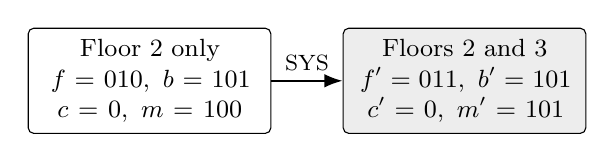
\begin{tikzpicture}[>=Latex,every node/.style={font=\small,align=center},
state/.style={draw,rounded corners=2pt,text width=2.8cm,minimum height=1.25cm,inner sep=4pt}]
\node[state] (before) at (0,0)
 {Floor 2 only\\$f=010,\ b=101$\\$c=0,\ m=100$};
\node[state,fill=black!7] (after) at (4.0,0)
 {Floors 2 and 3\\$f'=011,\ b'=101$\\$c'=0,\ m'=101$};
\draw[->,thick] (before.east)--node[above,font=\footnotesize]{SYS}(after.west);
\end{tikzpicture}\par\medskip
\small The movement disjunct $f'_3\land b_3$ holds.\\
Next $\operatorname{One}(f)$ fails: \textbf{no legal input remains}.
\caption{A reached Lift response disables ENV.
Table~\ref{tab:lift-prefix-main} gives its original-legal initialized prefix;
$f$, $b$ and $m$ are floor, button and monitor triples (order 1--3);
$c$ is cancellation. Here $b$ denotes buttons, not the helper.
This edge reuses the bad node; diagnostic
selection also acts at first creation.}
\label{fig:lift-admission}
\end{figure}

\paragraph{Source mechanism}
Lift T copies the trivial replacement listing's Boolean declarations,
initializers, safety clauses and response guarantees verbatim~\cite{degradation}.
Its only completion appends the same paper's omitted response-pattern
definition (Appendix~C.2.1), compiled into the logical SYS monitors below.
The outputs $f_1,f_2,f_3$ indicate floors; inputs $b_1,b_2,b_3$ are
buttons and $c$ is cancellation. Here $b_i$ denotes a button, distinct
from the helper $b$. The published listing labels \code{one\_floor} and
its three exclusivity clauses as \code{assumption}~\cite[Appendix~C.3.3,
lines~36--46]{degradation}; their conjunction is $\operatorname{One}(f)$.
Under the recorded translation, environment safety is
\[
\begin{aligned}
E_L={}&\operatorname{One}(f)\land\bigwedge_{i=1}^{3}
\bigl[(b_i\land f_i\Rightarrow\neg b_i')\\
&\qquad\land(b_i\land\neg f_i\land\neg c\Rightarrow b_i')\bigr],
\end{aligned}
\]
where $\operatorname{One}(f)$ requires exactly one \emph{current} floor.
The recorded translator keeps SYS/AUX-dependent invariants as current
ENV safety, without an initializer or primed copy. Thus the listing
fixes ownership and the translation fixes timing; neither is changed
by this reconstruction.
System safety conjoins $f_i\Rightarrow D_i$ for all three floors, where
\[
\begin{aligned}
D_1={}&(f'_1\land(\neg b_2\land\neg b_3\lor c))
       \lor(f'_2\land(b_2\lor b_3)),\\
D_2={}&(f'_1\land b_1)\lor(f'_2\land\neg b_1\land\neg b_3)\\
 &\lor(f'_3\land b_3)\lor(f'_2\land c),\\
D_3={}&(f'_3\land(\neg b_1\land\neg b_2\lor c))
       \lor(f'_2\land(b_1\lor b_2)).
\end{aligned}
\]
Every button and cancellation guard uses its current value. Thus $D_2$
permits both $100$ and $011$ when $b_1=b_3=1$; no conjunct forbids
extra true next floors. For each response obligation, SYS safety also requires
\[
 m_i'\leftrightarrow(m_i\lor b_i)\land\neg(f_i\lor c),
 \qquad i=1,2,3.
\]
These logical monitors are part of the source state; their justices are
$\G\F\neg m_i$. Initialization sets buttons $000$, floors $100$ and
monitors $000$, leaving $c$ free; ENV has no justices. Private selector
$j$ belongs only to the returned graph. Supplement~H retains the source.

\begin{table}[!ht]
\centering\small
\caption{Saved Lift prefix to Fig.~\ref{fig:lift-admission}: native node
IDs and private justice selector $j$. Rows are completed states; the next
row's $(b,c)$ supplies the next input. The helper stays false. The last
row is the bad node's construction predecessor, outside this prefix.}
\label{tab:lift-prefix-main}
\begin{tabular}{@{}rccccc@{}}\toprule
Node & Buttons $b$ & $c$ & Floors $f$ & Monitors $m$ & $j$\\\midrule
0   &000&0&100&000&0\\
10  &010&1&100&000&0\\
339 &001&1&010&000&0\\
438 &100&0&001&000&1\\
704 &101&0&010&100&2\\
680 &101&0&011&101&0\\\midrule
\multicolumn{6}{@{}l}{First-creation predecessor of node 680:}\\
668 &111&0&010&110&2\\\bottomrule
\end{tabular}
\end{table}

At node 704 in Table~\ref{tab:lift-prefix-main}, repeating the input is legal.
Figure~\ref{fig:lift-admission} shows the returned response $f'=011$:
its $f'_3\land b_3$ disjunct holds and the monitors update $100\to101$.
No SYS clause forbids the second true floor. In the successor,
$\operatorname{One}(f)$ fails, so all next inputs are illegal.
The table binds this edge to an original initializer and the graph's
actual private memory. The complete 154-state original-contract graph
is strict but non-cooperative. It violates Kind Definition~3~\cite[Sec.~4]{kind}:
an original-legal reachable prefix has no environment-fair continuation.
Current SYS variables in ENV safety are allowed by Kind's input
syntax~\cite[Sec.~3.1]{kind}. The same contract has the cooperative policy
below, yet the transformed game permits the bad node. Thus the failure
belongs to the selected extractor's fixed graph, not source infeasibility.
The selected raw arena fails the sufficient
language-inclusion condition for non-conflictingness~\cite[Eq.~(13c),
Theorem~3]{friendly}: a checked initialized lasso reaches helper true,
satisfies all SYS justices and violates the added ENV justice. This is a
selected-route output failure, not an abstract-theorem counterexample;
Supplement~V gives the precise bindings.

\paragraph{A positive source policy}
Let $\ell\in\{1,2,3\}$ be the unique current floor and let private
priority $d\in\{1,3\}$ start at 3, independently of graph selector $j$.
The following policy reads current buttons; the floor-2 tests are ordered:
\[
\begin{array}{ll}
\ell=1:&\ell'\gets2\text{ if }b_2\lor b_3,\text{ else }1;\\
\ell=3:&\ell'\gets2\text{ if }b_1\lor b_2,\text{ else }3;\\
\ell=2:&\ell'\gets d\text{ if }b_1\land b_3;\ 1\text{ if }b_1;\\
       &\qquad 3\text{ if }b_3;\ 2\text{ otherwise}.
\end{array}
\]
Set $f_i'\leftrightarrow(i=\ell')$, apply the stated monitor equation,
and set $d'=4-\ell'$ on departure from floor 2, keeping $d$ otherwise.
Each move satisfies a displayed movement disjunct. An unanswered button
persists until arrival or cancellation. Without cancellation, endpoint
priority can be lost at most once, so service occurs within four
transitions; arrival or cancellation clears the monitor on the next.
The middle floor is reached within one transition when requested.
Initialization and legal ENV persistence imply $m_i\Rightarrow b_i$
on every policy prefix. A permanently pending monitor would therefore
force a persistent uncancelled button, contradicting the service bound.
Thus all monitor justices hold from original initialization.

Every legal policy prefix retains $\operatorname{One}(f)$ and a legal
next input. Repeatedly taking $c'=1$ and
$b_i'=b_i\land\neg f_i\land\neg c$ is one ENV-safe infinite suffix;
there are no ENV justices. This proves cooperation under the same
reached policy memory, independently of a saved graph report.
The complete initialized graph has 128 nodes and 1,020 edges and passes
both checks. A separately checked extension also wins the complete
transformed game (Supplement~H). Neither result claims correctness
from arbitrary orphan-monitor states.


\paragraph{A matched selection diagnosis}
We audit the chain in Table~\ref{tab:route-evidence} directly.

One solve supplies the same model and memory objects to both extractors.
Saved checks establish equal winning region, stored fixed-point sets
$X,Y,Z$, initializers,
transition relations and ordered justices, with unchanged variable order.
For a candidate successor $t$ and Boolean helper $h$, define
\[
 Q(t)=h(t)\lor\exists e'\in E:\rho_e^{\rm native}(t,e')[h=0,h'=0].
\]
After the unchanged progress, goal and existing-node filters produce
$B$, the modified copy substitutes $B\cap Q$ when nonempty, otherwise
$B$, immediately before final response selection. Rank selection and
private-memory updates remain unchanged. This tests immediate input
availability, retaining helper-true candidates; complete graph audits
establish cooperation. Source equations match the helper-false relations
on all 1,048,576 original state pairs, initializers and ordered justices;
both auditors share compiler exports.

At the first creation of bad node 680, the final candidate floor set is
$B=\{011,100,101,110,111\}$ and $B\cap Q=\{100\}$.
The released extractor chooses $011$; the diagnostic selection chooses
$100$, which permits four next inputs. At the later reused edge in
Fig.~\ref{fig:lift-admission}, the existing-node filter leaves only
$011$. Thus the intervention acts during extraction, including first
creation, rather than replacing only the displayed reused edge.
Supplement~W gives the preceding filters and exact predecessor.

The initialized original-contract graphs each have 154 nodes, with
1,170 released and 1,176 preference edges. Both complete checkers classify the released graph as strict-only and
the preference graph as strict and cooperative
(Table~\ref{tab:route-evidence}). The matched output difference is at final selection, but that is not
the sole cause: the transformed game already permits the bad node.
The intervention is inactive in six successful controls. Counts include
two initial nodes and native memory; equal counts do not identify nodes.
Supplements~H and T retain calls, candidates, traces and certificates.

A separate contract control moves the floor-invariant clauses from
ENV/current to SYS/next constraints. Both graphs then coincide and pass
the audits. Ownership and timing change together, so this is a contract
sensitivity check, not evidence that the original contract needs changing
(Supplement~W).

\paragraph{Why this is a diagnostic contrast}
Constructed Polling has the safety assumption
$\neg poll\Rightarrow\neg ack'$, ENV justice $\G\F ack$, and SYS
justice $\G\F heartbeat$. An input remains available everywhere.
Normalized synthesis on the original nonblocking arena computes exact
$K=D$, yet the generic extractor returns a strict graph with terminal
cycle $poll=ack=0$ and no fair ENV continuation. The helper-based
released and selection-variant outputs also fail cooperation, with
unchanged responses. Hence availability selection and a correct existence
region do not certify a fixed graph. All three saved outputs fail the
complete cooperation check (Supplement~O).


\section{Admission and Existing Comparisons}\label{sec:replication}
The distinction in Section~\ref{sec:running-example} gives a concrete
admission rule: keep the source state and logical monitors fixed,
bind each candidate's private root, and install the first passing graph.
If all candidates fail or remain UNKNOWN, defer replacement without
inferring source infeasibility. Holding continues only while valid;
otherwise the bridge or revalidation condition in
Section~\ref{sec:running-example} applies. Changing the contract needs a
preserving refusal or a separate source argument.

\subsection{Complete fixed-graph checks}
The audit checks the selected root or required initial choices,
responses to every original-legal input, source safety, logical-monitor
and private-memory updates, strict liveness, and legal-prefix cooperation.
In the graph of checked legal responses, an \emph{ENV-accepting} strongly
connected component (SCC) contains a cycle and intersects every ENV justice.
Cooperation holds exactly when every reachable node can reach such an SCC.
Strict liveness requires that, for each SYS justice, removing the nodes
satisfying it from the already reachable graph leaves no ENV-accepting SCC. SCCs need not be bottom
components; a singleton needs a self-loop. Even with no ENV justices,
a cycle is required.

A model-based audit requires typed predicate correspondence; a direct
audit uses source equations. Original-contract views of helper-based
graphs keep the helper false and retain every original-legal input.
Missing correspondence or exhausted resources leaves the relevant decision
UNKNOWN; it does not invalidate an independent source certificate.

\subsection{Existing synthesis as a source of alternatives}\label{sec:cooperation}
Let $V=\nu X.(\mathit{Alive}\land\CPre(X))$, where $\mathit{Alive}$
means some original-legal next input exists and $\CPre(X)$ requires a
safe SYS response into $X$ for every such input. Every strict cooperative
strategy remains in $V$. If $V=\varnothing$, then $K=\varnothing$;
otherwise retain every original-legal input and all safe responses into
$V$, and split rounds into input/response edges to obtain a finite total
arena $H$. The reached states and residual strategies form a post-fixed point
of $\mathit{Alive}\land\CPre$; restriction retains their legal prefixes
and memory. Conversely all original-legal inputs are retained, and
$A\Rightarrow(G\land A)\equiv A\Rightarrow G$. Thus normalization
preserves $K$ (Supplement~L.2) and establishes the language premise
$L(H,G\land A)\subseteq L(H,A)$~\cite{cooperative,friendly}.
Justice labels occur only on completed states, with empty lists padded
by true. The round correspondence identifies final regions, not
extracted ranks (Supplements~A and L.2).

The cited four-fixed-point theorem supplies a prescribed rank/mode
witness inside $K$ and excludes every history-dependent strict
cooperative strategy outside it~\cite[Eq.~(18), Theorem~3,
Apps.~B.1--B.2]{friendly}. Our generic constructor has no established
binding to that strategy; every returned graph is audited separately.


\subsection{A paused replacement and its consequence}\label{sec:lift-episode}
\label{sec:runtime-admission}
Under the constructed old Lift restriction $\G\neg b_1$, inputs
$0010,0010$ in $(b_1,b_2,b_3,c)$ order reach native nodes
$0\to4\to524$. The paused state is
\[
(b_1b_2b_3,c,f_1f_2f_3,m_1m_2m_3)=(001,0,010,001),
\]
with an unanswered third-floor request. Removing the restriction retains
this valuation. Candidate node/selector pairs are native $524/1$,
normalized $72/1$, and selection variant $524/1$; IDs are graph-local,
and the normalized graph has no helper.

At all three pending boundaries in the old closure, the manager tries
native, normalized, then the selection variant until the first complete
pass. Coverage, safety, monitor/memory and SCC checks withhold native,
admit normalized and leave the third candidate untried. No source field,
monitor or runtime state object changes during selection. The displayed
case installs normalized root $72/1$ (Supplement~U.9).

Separate bounded executions compare all nine candidate/root pairs.
All serve the old request at step~1 and clear its monitor at~2.
The three retained-native executions later stop after eight commits,
with a new first-floor request pending and no legal input. The six
alternatives complete twelve commits and reach a fair loop. Later
continuity differs; service of the old request does not. Gated native
episodes instead remain paused with zero commits. Workloads were fixed
after diagnosis and before execution, not held out (Supplement~R).

Candidates are prepared beforehand. Gate measurements exclude synthesis:
4.448--5.207\,s for Patrol, and 0.039--0.059\,s per Lift candidate plus
0.357--0.481\,s shared loading/binding. These are bounded software
measurements, not latency guarantees (Supplement~U.4).


\subsection{What the fixed comparisons establish}
Table~\ref{tab:comparison-summary} keeps the input sets and their
selection rules separate. Existing normalized synthesis supplies admitted
graphs for every cooperatively feasible contract in the two fixed rosters:
eight of eleven reconstructed listings and twelve of fourteen public inputs. These are separate
route runs, not matched extractions, and establish available alternatives
rather than selection-variant necessity or comparative superiority.

\begin{table*}[t]
\centering\small
\caption{Existing comparisons, with distinct units and selection rules.
An admitted graph passes strictness and legal-prefix cooperation checks.
All outcomes, exclusions and UNKNOWNs are retained in Supplements~E, H, T and Y.}
\label{tab:comparison-summary}
\begin{tabular}{@{}L{43mm}L{78mm}L{43mm}@{}}\toprule
Input set and selection & Saved results & What the comparison establishes\\\midrule
All 11 replacement listings in five published examples' appendices;
reconstructed. &
Selected: 7 admitted, 2 strict-only, 1 raw negative,
1 correspondence UNKNOWN. Normalized: 8 admitted; 3 independently
confirmed empty-$V$ stops before solving. &
Existing normalized synthesis succeeds on all 8 feasible listings.
Correlated reconstructions, not historical executions.\\[4pt]
14 unchanged public inputs: all available certified carriers with at most
4,096 states; no region or output filtering. &
Selected: 11 admitted, 2 strict-only, 1 resource UNKNOWN.
Normalized/cooperative Slugs: 12 admitted and 2 negative each.
Original nonblocking strict: 12 admitted, 1 strict-only, 1 negative. &
Four routes, 56 recorded input/route outcomes. A bounded certified roster;
no population or performance inference.\\[4pt]
Stopped public inventory: 425 byte-distinct units, 70 model completions,
59 checker-certified models. &
Complete literal relations: 49 satisfy $W\subseteq C$; 10 lose strict
states. Exact loss finishes on 9, with no lost $K$ state; 1 remains
resource UNKNOWN. All 10 lack cooperative initialization. &
An explicit preservation diagnostic with negative results. Counts do not
transfer automatically to syntactic exports or estimate incidence.\\[4pt]
7 fixed cooperative-positive inputs~\cite{fixedsevennative2026} from the certified inventory;
old $W=K$ and literal preservation known. &
14 native strict queries and 198,672 typed-state comparisons: source $W$
equals old symbolic $W=K$
and the route source view in all 7; both initial judgments true. &
3 helper-active GyroAspect variants; 4 identity/skip controls.
No loss or gain in this selected set; no general preservation claim.\\\bottomrule
\end{tabular}
\end{table*}


The eleven listings come from five correlated examples; T and P denote
trivial and preferred replacements. For the selected route, Lift~T is the
only feasible contract with a failed cooperative output. The other unadmitted listings have empty
cooperative regions: Arbiter~P is strict-only, Minepump~P is raw-negative,
and Lift~P has unknown route correspondence. A raw negative need not be a
source refusal. Supplements~H (Tables~6--7) and T (Table~25) give the
candidate and route results.

The public roster's two strict-only outputs are PCar058, whose
cooperative region is empty, and Elevator032, whose nonempty cooperative
region fails initialization. Neither is a feasible-contract counterexample.
Resource-UNKNOWN SmartHome1~223 is admitted by all three alternatives
(Supplement~T).

\paragraph{Selection, stopping and negative results}
The public inventory contains 425 byte-distinct source units, including
two pattern libraries. Representative archive-path order with per-input caps of 60\,s,
512\,MiB heap and 128\,MiB direct memory produced 70 completed original models, 107 resource UNKNOWNs, 54 technical
UNKNOWNs, one integrity UNKNOWN and 193 unattempted inputs. A BDD-file cap
followed by a process-cleanup permission failure stopped the run. Of the
70 completions, two exceeded the checker's 64-variable limit and nine
failed array-metadata roster checks; all remaining 59 certified models
entered the literal-preservation analysis, without outcome filtering.
This is a stopped, resource- and certification-conditioned cohort.

Among its ten strict-preservation losses, all contracts already lack
cooperative initialization. Nine exact-loss calculations completed: seven
have empty $K$ and two preserve every $K$ state; the tenth remains UNKNOWN.
Thus this cohort contains no confirmed cooperative-initialization loss,
and it supplies no incidence estimate. The separate Vehicle witness and
constructed Polling control are outside these denominators.
Selected Humanoid044 also has source $V=K=\varnothing$; its guard study
does not establish a cooperative rescue (Supplement~D).

\paragraph{Accessible evidence and shared dependencies}
The archives~\cite{savedartifact,newartifact,pendingartifact,diagnosticartifact,continuationartifact}
retain sources, graphs, certificates and saved-data replay instructions.
Lift's separate decoders and source-equation audits share compiler exports;
region and memory checks share a decoder. Patrol combines source, raw-BDD
and explicit-set checks. Neither compiler independence nor external
reproduction follows. Supplements~U--Y distinguish native execution,
saved membership, graph audits and source proofs.


\section{Scope and Related Work}\label{sec:discussion}
\paragraph{Scope of the decision}
Admission assumes prepared candidates and a valid hold. Changing physical
state requires a verified bridge or revalidation. Change detection and
automatic candidate generation remain outside this implementation.

\balance
Strict preservation alone does not imply cooperation. Source ENV justice
may be impossible, and a helper flip itself defeats the added justice.
Normalization after conversion need not restore cooperation (Supplement~L.2).

\paragraph{Relation to prior work}
Multi-tier control, exploration, weakening, recovery, interpolation
and permissive assumptions~\cite{dippolito2014multitier,keegan2022discovery,weakening2023,graceful2024,cavezza2017interpolation,anand2023apa}
construct adaptation choices; our diagnoses test whether retaining the
original contract is already justified.
Cooperative synthesis~\cite{cooperative,friendly} certifies its prescribed
construction. IROS's middle-fixed-point restrictions block all six
priorities~\cite[author appendix, p.~9]{iros}; Lift retains response $100$
and localizes the matched difference to final selection.
Best-effort GR(1) retains fairness opportunities~\cite{besteffort};
acceleration preserves a language-inclusion premise~\cite[Sections~2.3,~4.1]{accelerating}.
The implemented guard's complete form preserves strict
winning~\cite{spectrarelease2024}; our results characterize other encodings.
Well-separation classifies targeted assumption violations~\cite[Section~6.3]{wellsep}.
Dynamic-update synthesis constructs bridges~\cite{nahabedian2020dynamic,dupdate};
runtime verification retains monitors~\cite{runtimeverification2023}.
Our fixed-entry admission decision precedes any needed changing-state bridge.


\section{Conclusion}\label{sec:conclusion}
At a retained source state, the exact theorem and Vehicle/Patrol identify
continuation loss under Boolean-helper encodings. Lift separates fixed-output
admission. Existing normalized synthesis and complete graph audits support
retaining feasible contracts and admitting qualified candidates. Deployment
frequency and general repair effectiveness remain open.


\section*{Acknowledgments}
OpenAI Codex~\cite{codex} assisted with drafting throughout this paper,
formal reasoning (Sections~\ref{sec:running-example}--\ref{sec:replication}),
and experiment design, derivation, implementation, execution, auditing
and analysis (Sections~\ref{sec:evaluation}--\ref{sec:replication}).
Claude (Fable 5.1) and ChatGPT (GPT-6 Pro) reviewed main-paper drafts;
Fable also reviewed supplement drafts and a primary paper. The
supplement's acknowledgments detail the workflow and limitations.

\clearpage
\nobalance
\IEEEtriggeratref{15}
\begin{thebibliography}{25}
\bibitem{specrepair}T. Buckworth, D. Alrajeh, J. Kramer, and S. Uchitel, ``Adapting specifications for reactive controllers,'' in \emph{SEAMS}, 2023, pp. 1--12. doi: \href{https://doi.org/10.1109/SEAMS59076.2023.00012}{10.1109/SEAMS59076.2023.00012}.
\bibitem{degradation}T.-A. Georgescu, D. Alrajeh, and S. Uchitel, ``Learning to adapt GR(1) specifications through degradation,'' arXiv:2609.12231v1, Sept. 2026. \url{https://arxiv.org/abs/2609.12231v1}.
\bibitem{dupdate}G. Amram, S. Maoz, I. Segall, and M. Yossef, ``Dynamic update for synthesized GR(1) controllers,'' in \emph{ICSE}, 2022, pp. 786--797. doi: \href{https://doi.org/10.1145/3510003.3510054}{10.1145/3510003.3510054}.
\bibitem{spectrarelease2024}Software Modeling Lab, ``Spectra Tools: Released Game-Model Bundle,'' version 1.0.0.202402072123, 2024. Bundled source: \code{PitermanSemanticReduction}. \url{https://smlab.cs.tau.ac.il/syntech/spectra/tools/update/plugins/tau.smlab.syntech.gamemodel_1.0.0.202402072123.jar}.
\bibitem{artifactrepository}Anonymous artifact contributors, \emph{Continuation Preservation: Research Artifact}, Oct.~2026. \url{https://github.com/research-artifact-archive/seams2027}. Document/layout snapshot: \href{https://github.com/research-artifact-archive/seams2027/tree/reader-layout-20261024-v1}{\nolinkurl{reader-layout-20261024-v1}}.
\bibitem{gr1}R. Bloem, B. Jobstmann, N. Piterman, A. Pnueli, and Y. Sa'ar, ``Synthesis of Reactive(1) Designs,'' \emph{J. Comput. Syst. Sci.}, vol. 78, no. 3, pp. 911--938, 2012. doi: \href{https://doi.org/10.1016/j.jcss.2011.08.007}{10.1016/j.jcss.2011.08.007}.
\bibitem{kind}A. Gorenstein, S. Maoz, and J. O. Ringert, ``Kind controllers and fast heuristics for non-well-separated GR(1) specifications,'' in \emph{ICSE}, 2024. doi: \href{https://doi.org/10.1145/3597503.3608131}{10.1145/3597503.3608131}.
\bibitem{cooperative}R. Bloem, R. Ehlers, and R. K\"onighofer, ``Cooperative reactive synthesis,'' in \emph{ATVA}, 2015, pp. 394--410. doi: \href{https://doi.org/10.1007/978-3-319-24953-7_29}{10.1007/978-3-319-24953-7\_29}.
\bibitem{friendly}R. Majumdar, N. Piterman, and A.-K. Schmuck, ``Environmentally-friendly GR(1) synthesis,'' in \emph{TACAS}, 2019, pp. 229--246. doi: \href{https://doi.org/10.1007/978-3-030-17465-1_13}{10.1007/978-3-030-17465-1\_13}. Extended proofs: \url{https://arxiv.org/abs/1902.05629}.
\bibitem{newartifact}Anonymous, \emph{Certificate and Finite-Study Evidence}, version certificate-finite-evidence-20261023-v2, Oct.~2026. \url{https://github.com/research-artifact-archive/seams2027/tree/certificate-finite-evidence-20261023-v2}.
\bibitem{spectra}S. Maoz and J. O. Ringert, ``Spectra: a specification language for reactive systems,'' \emph{Software and Systems Modeling}, vol. 20, pp. 1553--1586, 2021. doi: \href{https://doi.org/10.1007/s10270-021-00868-z}{10.1007/s10270-021-00868-z}.
\bibitem{vehicleartifact}Anonymous, \emph{Vehicle188 Native Strict Evidence}, version vehicle188-native-evidence-20261024-v1, Oct.~2026. \url{https://github.com/research-artifact-archive/seams2027/blob/vehicle188-native-evidence-20261024-v1/VEHICLE188_NATIVE_EVIDENCE.md}.
\bibitem{vehiclewholeartifact}Anonymous artifact contributors, \emph{Vehicle188 whole-region saved evidence}, version vehicle188-whole-region-evidence-20261024-v1, Oct.~2026. \url{https://github.com/research-artifact-archive/seams2027/blob/vehicle188-whole-region-evidence-20261024-v1/VEHICLE188_WHOLE_REGION_EVIDENCE.md}.
\bibitem{kindartifact}A. Gorenstein, S. Maoz, and J. O. Ringert, ``Artifact for ICSE'24 paper: Kind Controllers and Fast Heuristics for Non-Well-Separated GR(1) Specifications,'' Zenodo, v3, 2024. doi: \href{https://doi.org/10.5281/zenodo.10553249}{10.5281/zenodo.10553249}.
\bibitem{fixedsevennative2026}Anonymous artifact contributors, \emph{Fixed-seven native saved-data evidence}, version fixed-seven-native-evidence-20261024-v1, Oct.~2026. \url{https://github.com/research-artifact-archive/seams2027/blob/fixed-seven-native-evidence-20261024-v1/FIXED_SEVEN_NATIVE_EVIDENCE.md}.
\bibitem{savedartifact}Anonymous, \emph{Saved Controller Evidence}, version intruder-bounded-evidence-20261021-v1, Oct.~2026. \url{https://github.com/research-artifact-archive/seams2027/tree/intruder-bounded-evidence-20261021-v1}.
\bibitem{pendingartifact}Anonymous, \emph{Pending-Work Native Handoff Evidence}, version pending-native-handoff-evidence-20261023-v2, Oct.~2026. \url{https://github.com/research-artifact-archive/seams2027/tree/pending-native-handoff-evidence-20261023-v2}.
\bibitem{diagnosticartifact}Anonymous, \emph{Pending Diagnostic Evidence}, version pending-diagnostic-evidence-20261023-v1, Oct.~2026. \url{https://github.com/research-artifact-archive/seams2027/tree/pending-diagnostic-evidence-20261023-v1}.
\bibitem{continuationartifact}Anonymous, \emph{Continuation Evidence}, version continuation-evidence-20261024-v1, Oct.~2026. \url{https://github.com/research-artifact-archive/seams2027/blob/continuation-evidence-20261024-v1/CONTINUATION_EVIDENCE.md}.
\bibitem{dippolito2014multitier}N. D'Ippolito, V. Braberman, J. Kramer, J. Magee, D. Sykes, and S. Uchitel, ``Hope for the best, prepare for the worst: Multi-tier control for adaptive systems,'' in \emph{ICSE}, 2014, pp. 688--699. doi: \href{https://doi.org/10.1145/2568225.2568264}{10.1145/2568225.2568264}.
\bibitem{keegan2022discovery}M. Keegan, V. Braberman, N. D'Ippolito, N. Piterman, and S. Uchitel, ``Control and discovery of environment behaviour,'' \emph{IEEE Transactions on Software Engineering}, vol. 48, no. 6, pp. 1965--1978, 2022. doi: \href{https://doi.org/10.1109/TSE.2020.3044532}{10.1109/TSE.2020.3044532}.
\bibitem{weakening2023}S. Chu, E. Shedden, C. Zhang, R. Meira-G\'oes, G. A. Moreno, D. Garlan, and E. Kang, ``Runtime resolution of feature interactions through adaptive requirement weakening,'' in \emph{SEAMS}, 2023, pp. 115--125. doi: \href{https://doi.org/10.1109/SEAMS59076.2023.00025}{10.1109/SEAMS59076.2023.00025}.
\bibitem{graceful2024}S. Chu, J. Koe, D. Garlan, and E. Kang, ``Integrating graceful degradation and recovery through requirement-driven adaptation,'' in \emph{SEAMS}, 2024, pp. 122--132. doi: \href{https://doi.org/10.1145/3643915.3644090}{10.1145/3643915.3644090}.
\bibitem{cavezza2017interpolation}D. G. Cavezza and D. Alrajeh, ``Interpolation-based GR(1) assumptions refinement,'' in \emph{TACAS}, 2017, pp. 281--297. doi: \href{https://doi.org/10.1007/978-3-662-54577-5_16}{10.1007/978-3-662-54577-5\_16}.
\bibitem{anand2023apa}A. Anand, K. Mallik, S. P. Nayak, and A.-K. Schmuck, ``Computing adequately permissive assumptions for synthesis,'' in \emph{TACAS}, 2023, pp. 211--228. doi: \href{https://doi.org/10.1007/978-3-031-30820-8_15}{10.1007/978-3-031-30820-8\_15}.
\bibitem{iros}R. Ehlers, R. K\"onighofer, and R. Bloem, ``Synthesizing cooperative reactive mission plans,'' in \emph{IEEE/RSJ International Conference on Intelligent Robots and Systems (IROS)}, 2015, pp. 3478--3485. doi: \href{https://doi.org/10.1109/IROS.2015.7353862}{10.1109/IROS.2015.7353862}. Author version with appendix: \url{https://www.ruediger-ehlers.de/papers/iros2015.pdf}.
\bibitem{besteffort}S. Liu, Y. Zhang, C. Hu, and W. Dong, ``Best-effort GR(1) synthesis: Exploiting environmental cooperation under unrealizability,'' in \emph{ASE}, 2026, pp. 1806--1818. doi: \href{https://doi.org/10.1145/3832783.3837439}{10.1145/3832783.3837439}.
\bibitem{accelerating}S. Liu and W. Dong, ``Accelerating kind realizability: A multi-stage incremental realizability checking framework,'' in \emph{FM}, 2026, pp. 240--258. doi: \href{https://doi.org/10.1007/978-3-032-26204-2_13}{10.1007/978-3-032-26204-2\_13}.
\bibitem{wellsep}S. Maoz and J. O. Ringert, ``On well-separation of GR(1) specifications,'' in \emph{FSE}, 2016, pp. 362--372. doi: \href{https://doi.org/10.1145/2950290.2950300}{10.1145/2950290.2950300}.
\bibitem{nahabedian2020dynamic}L. Nahabedian, V. Braberman, N. D'Ippolito, S. Honiden, J. Kramer, K. Tei, and S. Uchitel, ``Dynamic update of discrete event controllers,'' \emph{IEEE Transactions on Software Engineering}, vol. 46, no. 11, pp. 1220--1240, 2020. doi: \href{https://doi.org/10.1109/TSE.2018.2876843}{10.1109/TSE.2018.2876843}.
\bibitem{runtimeverification2023}M. Carwehl, T. Vogel, G. N. Rodrigues, and L. Grunske, ``Runtime verification of self-adaptive systems with changing requirements,'' in \emph{SEAMS}, 2023, pp. 104--114. doi: \href{https://doi.org/10.1109/SEAMS59076.2023.00024}{10.1109/SEAMS59076.2023.00024}.
\bibitem{codex}OpenAI, \emph{Codex}, 2026. Accessed Oct.~23, 2026. \url{https://openai.com/codex/}.
\end{thebibliography}

\end{document}
